\hypertarget{a-suxedntese-pictuxf3rica-do-final-do-suxe9culo}{%
\subsection{A síntese pictórica do final do
século}\label{a-suxedntese-pictuxf3rica-do-final-do-suxe9culo}}

O próprio Meirelles, em suas telas da Guerra do Paraguai, acabaria se
afastando do paradigma documental e se aproximando da estética romântica
do sublime, mas nunca chegou a aplicá-la a vistas urbanas, tendo se
concentrado na pintura histórica e alegórica até o final de sua
carreira. Assim como na Capital, foi a atuação dos artistas de origem
estrangeira nas províncias --- no caso, imigrantes e seus descendentes,
em vez de viajantes ---, não comprometidos com as estruturas de poder ou
de ensino estabelecidas, que estimulou o desenvolvimento de abordagens
não documentais na iconografia urbana.

A produção de Nicola Antonio Facchinetti (1824--1900) no Rio de Janeiro,
de Pedro Weingärtner (1853--1929) no Sul do Brasil, e de seu coetâneo
Benedito Calixto em São Paulo sintetiza o percurso da iconografia urbana
brasileira no final do século XIX. Facchinetti, o mais velho dos três, e
chegando já adulto ao Brasil, atuou na continuidade da tradição
romântica da vista sublime, na qual a cidade se curva à escala da
natureza.

Weingärtner, nascido em Porto Alegre, conciliou sua formação nas escolas
acadêmicas da Europa com a temática realista que então competia com o
impressionismo pelo título de vanguarda. Seu registro da fundação de
Nova Veneza (Santa Catarina), intitulado Vida nova (1893, Figura
\ref{fig:weingaertner}), sinaliza uma inflexão nas vistas de cidades
brasileiras. Iniciando sua carreira quanto Meirelles já era
nacionalmente consagrado, ele não sentiu a mesma necessidade de se
acomodar num tipo iconográfico convencional, mas tampouco se aproximou
da estética romântica que valorizava a natureza dominante. Sua
composição ``meticulosamente estudada'' \autocite{carvalho:2008paisagem}
equilibra o povoado incipiente e a natureza como fundo, ressaltando um
episódio humano em primeiro plano. Trata-se de uma abordagem que
subverte tanto a dominância da natureza, cara aos românticos, quanto a
hierarquia do panorama documental, destinada a exaltar as sedes urbanas
do poder político e relegando as personagens do povo a detalhes de
ambientação.

\begin{figure}
\hypertarget{fig:weingaertner}{%
\centering
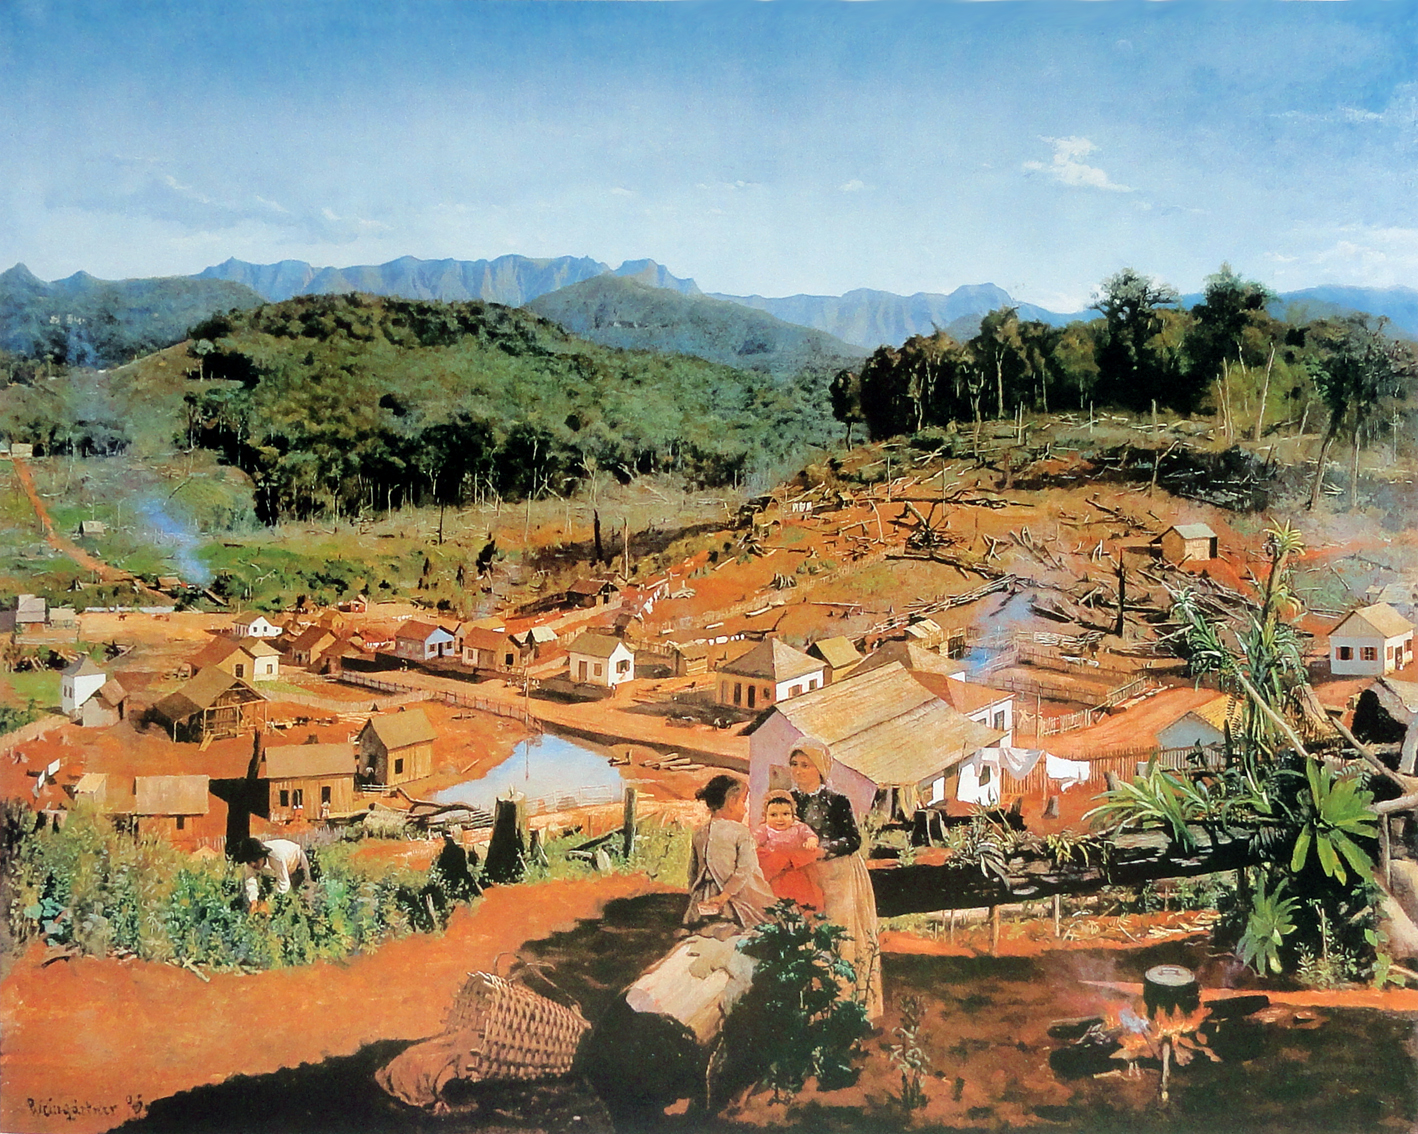
\includegraphics{figures/Pedro_Weingaertner_-_Vida_nova_-_1893.jpeg}
\caption{Pedro Weingärtner (1853--1929). Vida nova,
1893}\label{fig:weingaertner}
}
\end{figure}

Calixto, luso-brasileiro e paulista, destacou-se pelas vistas do litoral
de seu estado, seja no gênero de paisagem ou no da pintura histórica.
Sua canônica representação da Proclamação da República (1893), apesar de
moldada, pela dramatização dos acontecimentos, no triunfalismo
militarista, reatualizou a tipologia documental na tradição de Nicolas
Taunay. A tela (Figura \ref{fig:calixto}) apresenta um espaço urbano
circunscrito, sem ênfase na sua inserção na natureza, servindo como
fundo cênico para um acontecimento histórico. O conjunto da obra de
Calixto transita entre as vistas contemporâneas e o gênero histórico.
Diferentemente do ambiente artístico do início do século XIX, porém, não
há, na produção de Calixto, separação estanque entre os gêneros
pictóricos. Sua atuação remete à prática clássica de inserção de cenas
históricas ou bíblicas em exuberantes paisagens, que, de resto, havia
sido aplicada por Taunay pai no Rio de Janeiro. Por outro lado, a série
de pinturas de Santos e São Vicente, onde residia, quando tomada como
conjunto sobrepõe as múltiplas leituras da vista urbana documental, da
representação de cenas históricas, assim como reminiscências do tema
romântico da natureza pujante.

\begin{figure}
\hypertarget{fig:calixto}{%
\centering
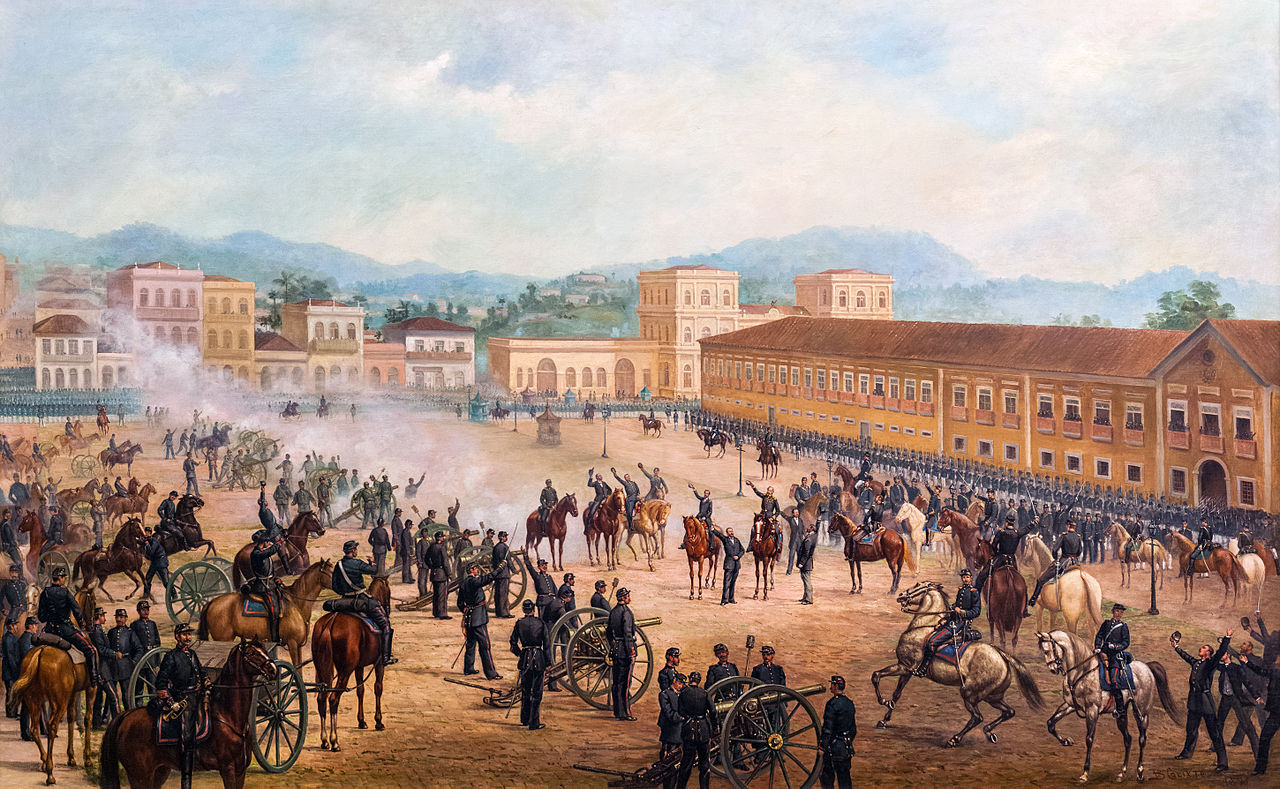
\includegraphics{figures/Proclamacao_da_Republica_by_Benedito_Calixto_1893.jpeg}
\caption{Benedito Calixto (1853--1927). Proclamação da República,
1893}\label{fig:calixto}
}
\end{figure}

A síntese operada nessa combinação de abordagens marca, entretanto, o
canto do cisne da vista urbana enquanto gênero misto de artístico e
documental --- para a geração de José Washington Rodrigues (1891--1957),
a recepção de obras semelhantes terminaria por recair exclusivamente no
seu caráter informativo, ao passo que os modernistas enfatizariam
exclusivamente o aspecto plástico das suas próprias representações de
cidades.
